\begin{figure}

\mode
<article>

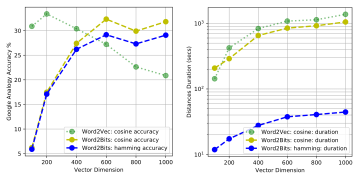
\includegraphics{word2bits-speed}

\vspace{-0.8cm}

\caption
  [The accuracy and speed of using fast approximate bitwise arithmetic
   on the English word analogy task]%
  {The accuracy (left) and speed (right) of using fast approximate
   bitwise arithmetic and slow floating point arithmetic on the English word
   analogy task. Reproduced with permission. \cite[Figure 3.8]{stefanik2019semantic}}

\protect\index[subject]{word analogy}

\mode
<presentation>

\scalebox{0.75}{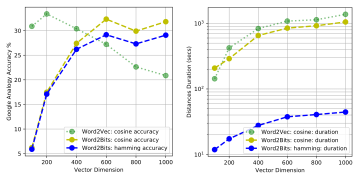
\includegraphics{word2bits-speed}}

\vspace{-0.4cm}

\caption
  {The accuracy (left) and speed (right) of using fast approximate
   bitwise arithmetic and slow floating point arithmetic on the English word
   analogy task. -- \textcite[Figure 3.8]{stefanik2019semantic}}

\mode
<all>

\label{fig:quantized-token-embeddings-with-fast-bitwise-arithmetic}
\end{figure}
